\begin{frame}
	\frametitle{Steady State}
		\textbf{Steady state neutron flux (with \gls{DNP} drift)}
		\begin{columns}
			\column{5cm}
			\begin{figure}
				\small
				\centering
				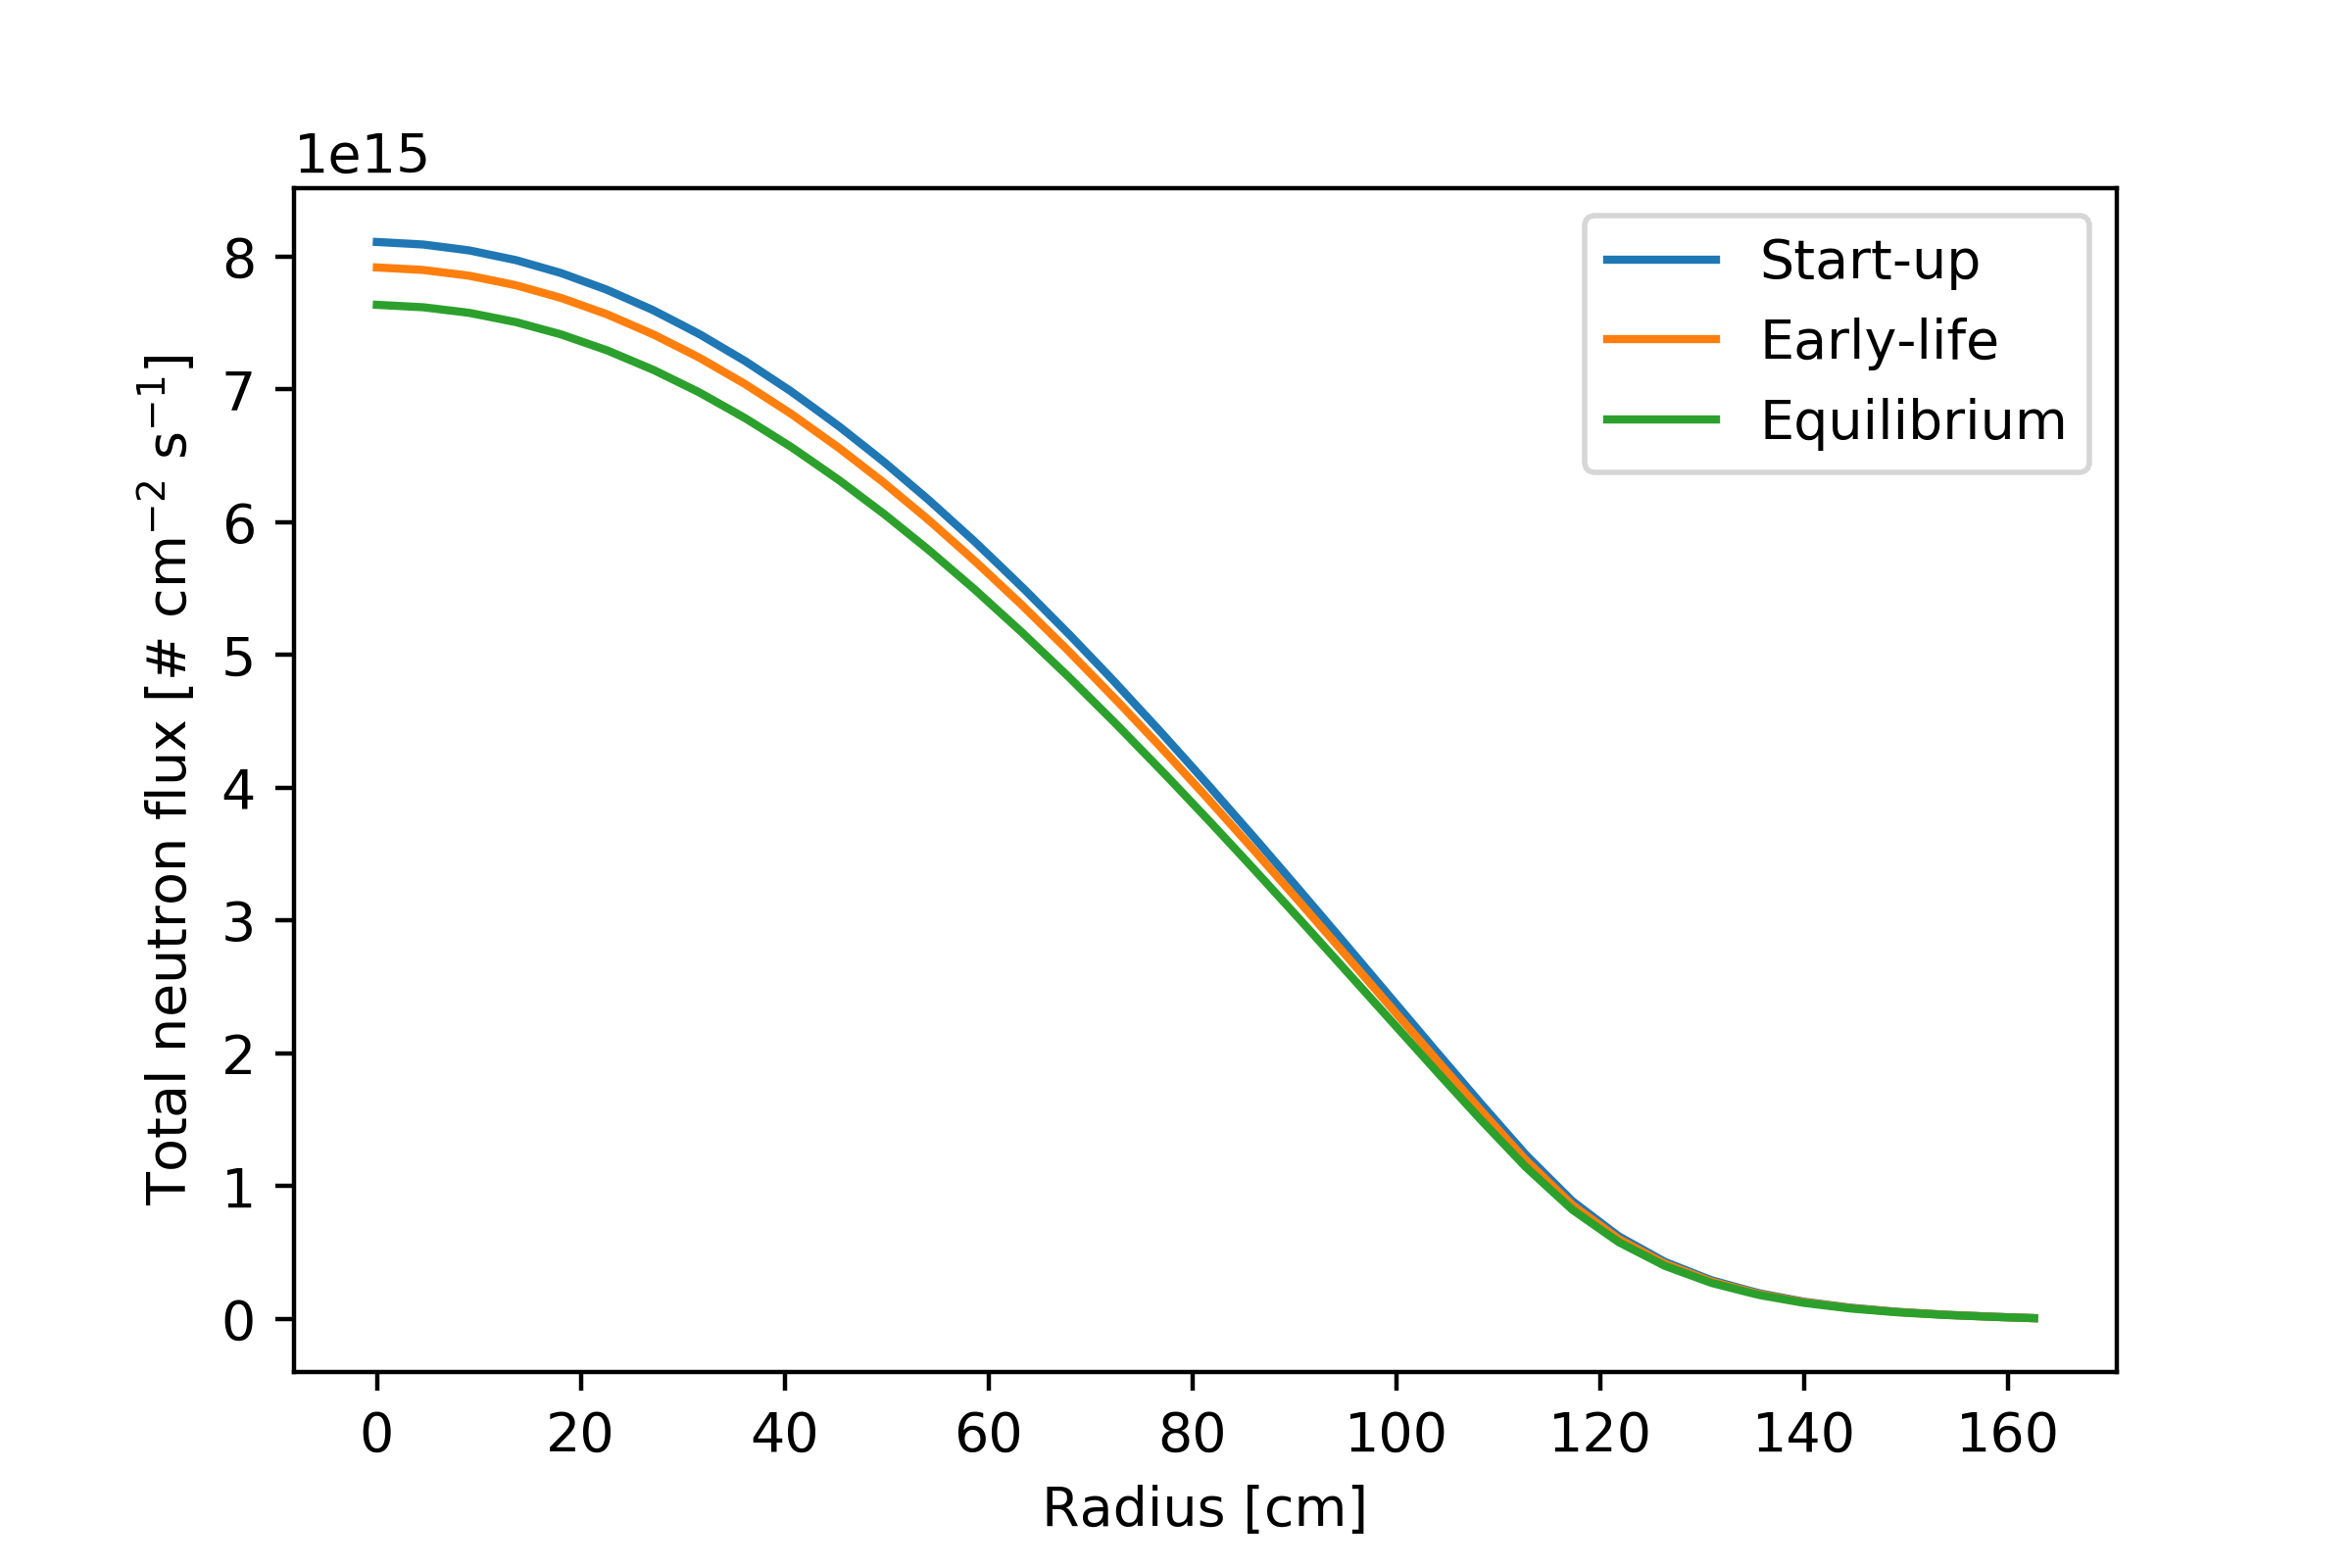
\includegraphics[width=\textwidth]{../paper/figures/totalflux}
				\caption{\small Total radial neutron flux at reactor
				half-height, for start-up, early-life, and equilibrium fuel
				compositions.}
				\label{fig:totalflux}
			\end{figure}
			\column{5cm}
			\begin{figure}
				\small
				\centering
				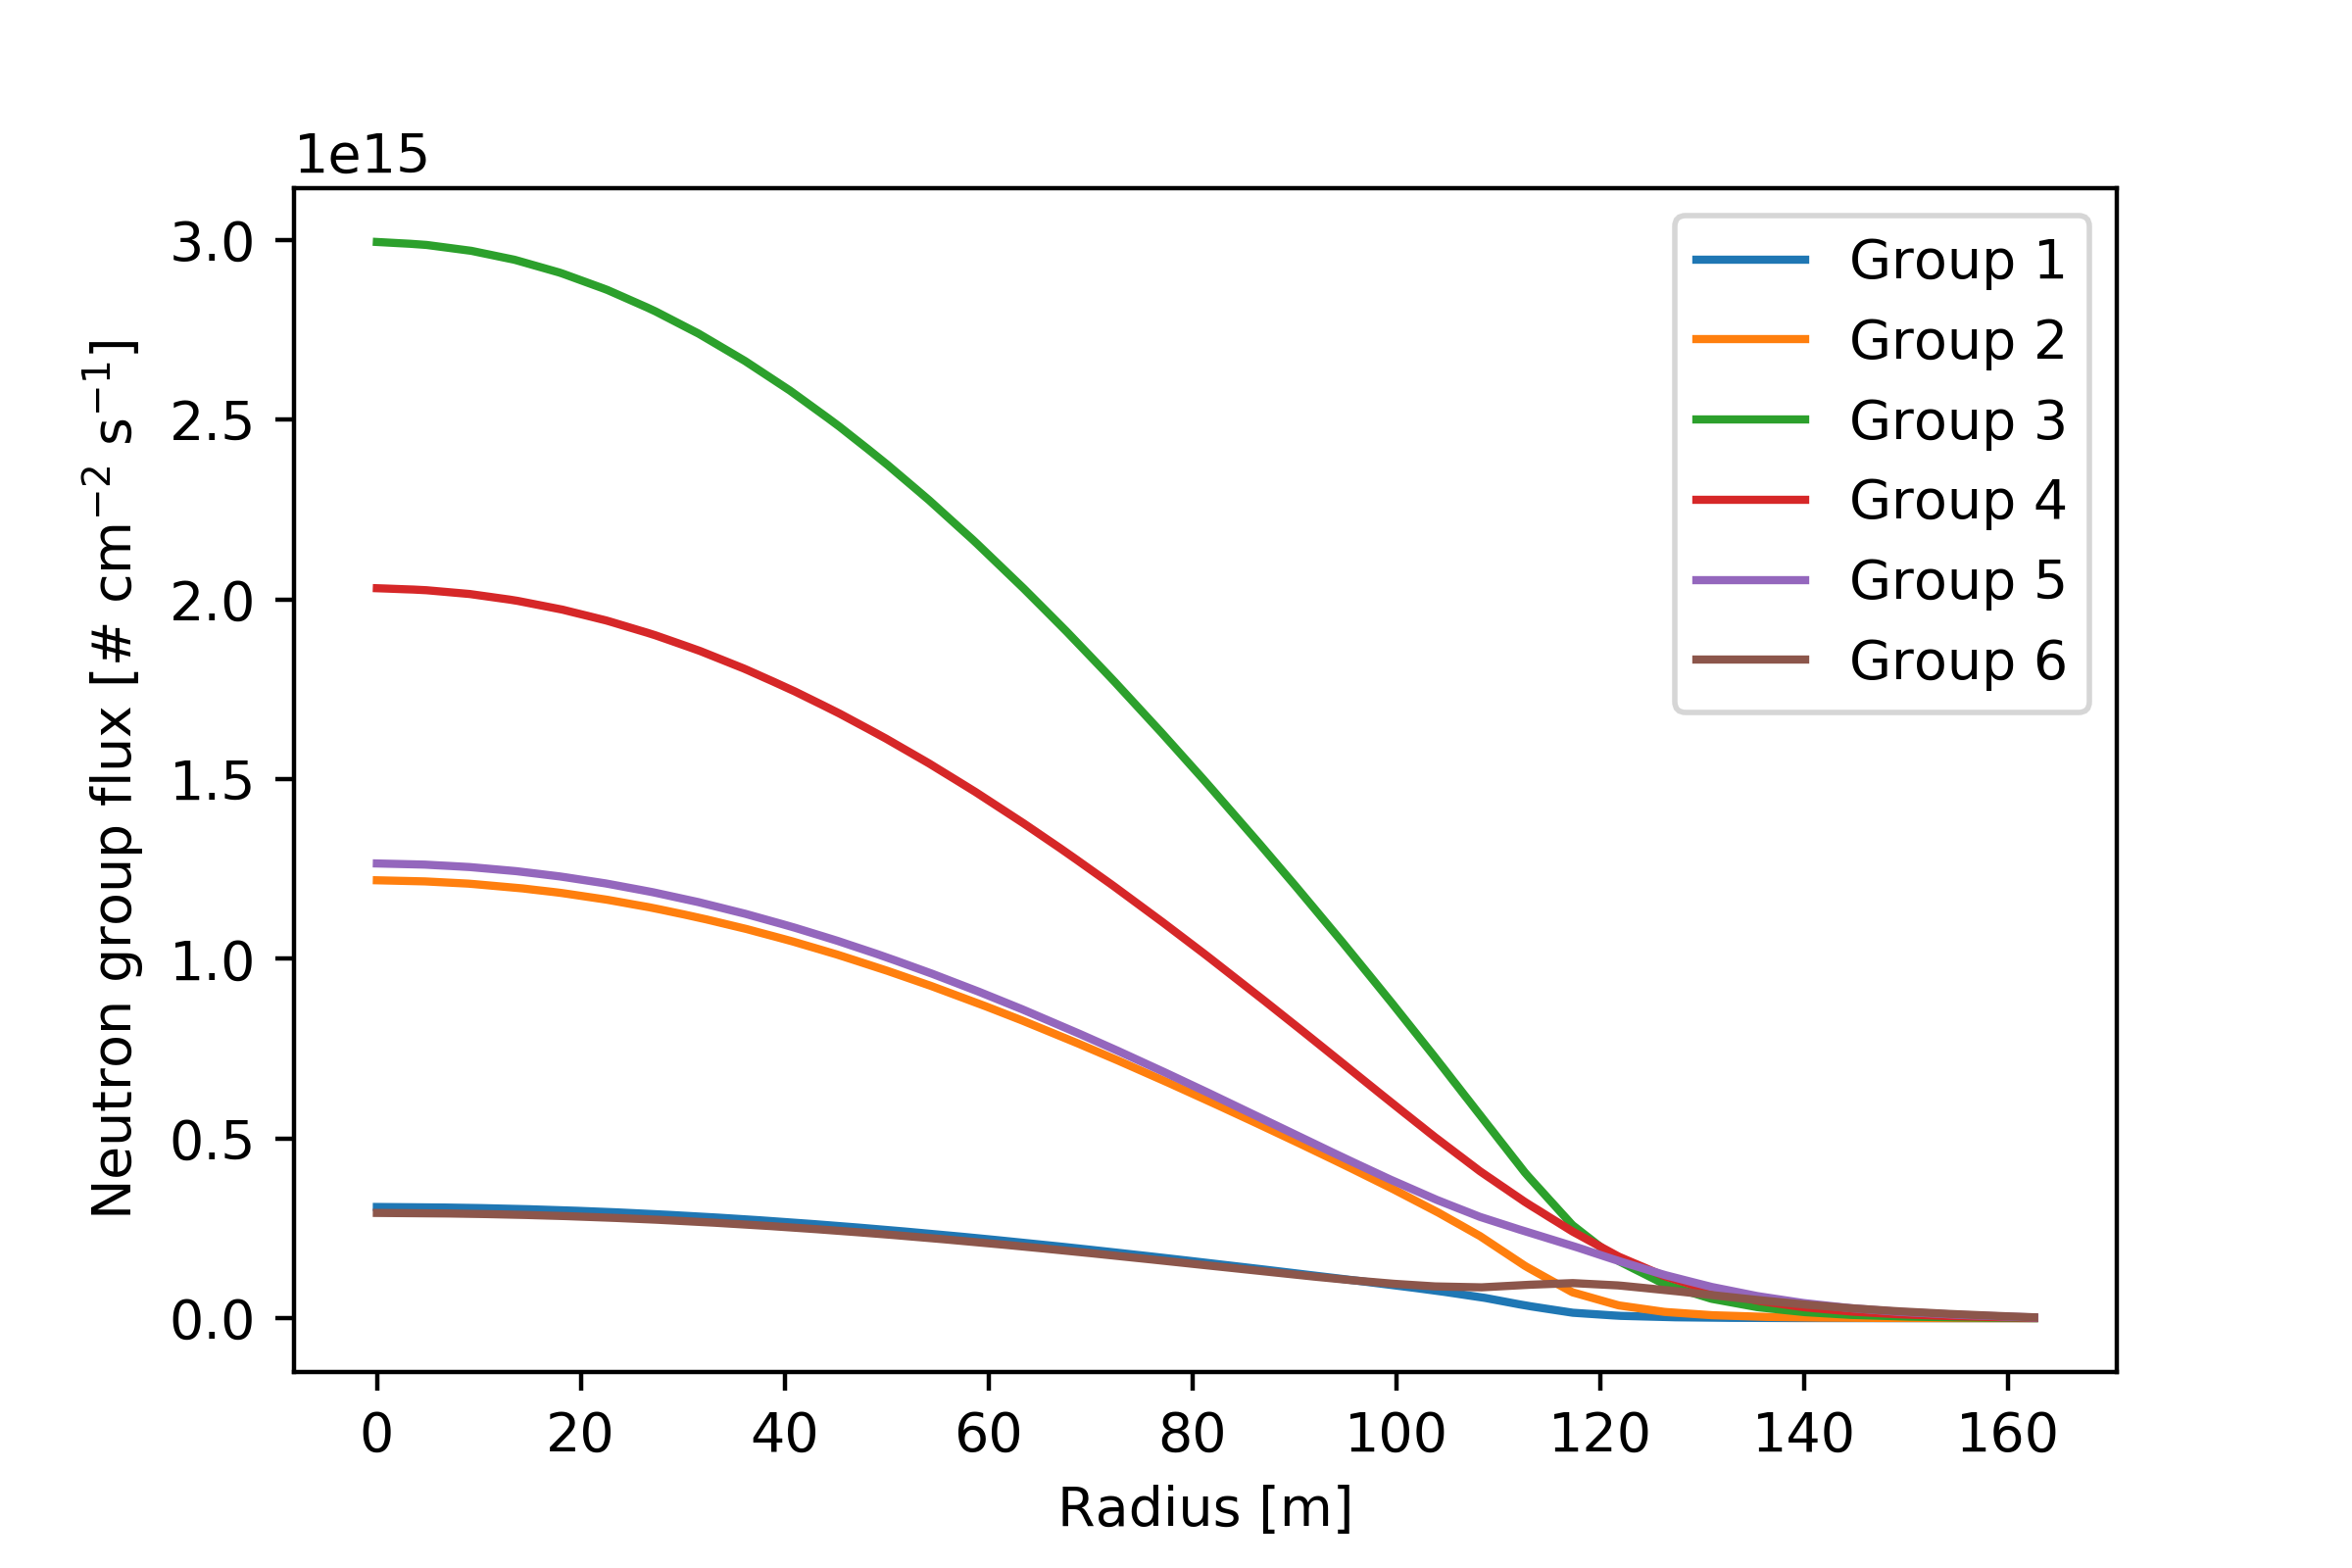
\includegraphics[width=\textwidth]{../paper/figures/stflux}
				\caption{\small Neutron group fluxes at reactor half-height, for
				start-up, early-life, and equilibrium fuel compositions.}
				\label{fig:stflux}
			\end{figure}
		\end{columns}
		\begin{itemize}
			\item Peak neutron flux is close to $8.6 \times 10^{15}$ cm$^{-2}$
			s$^{-1}$ reported by Fiorina et al.
			\cite{fiorina_investigation_2013}
		\end{itemize}
\end{frame}

\begin{frame}
	\frametitle{Steady State}
		\textbf{Steady state temperature distribution}
		\begin{columns}
			\column{12cm}
			\begin{figure}
				\small
				\centering
				\begin{subfigure}
					\centering
					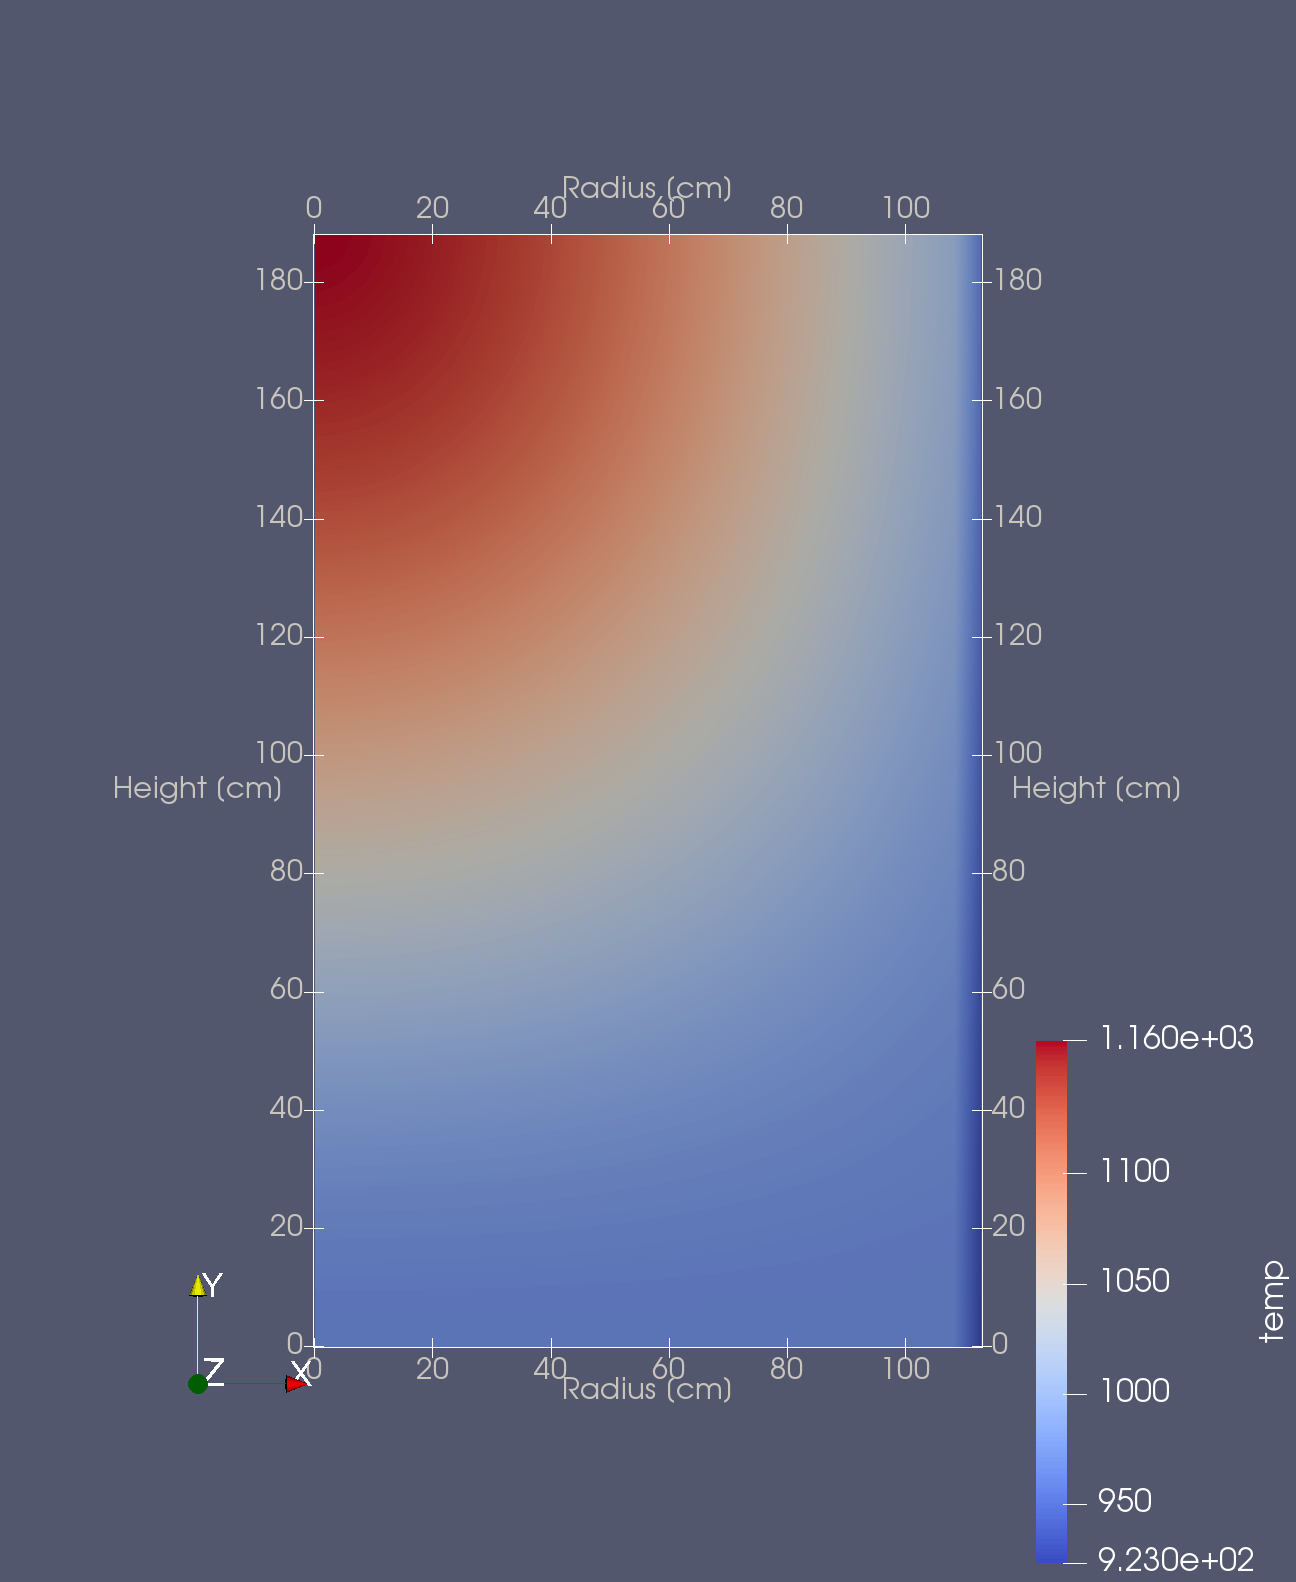
\includegraphics[width=.3\textwidth]{../paper/figures/sttemp}
				\end{subfigure}
				\begin{subfigure}
					\centering
					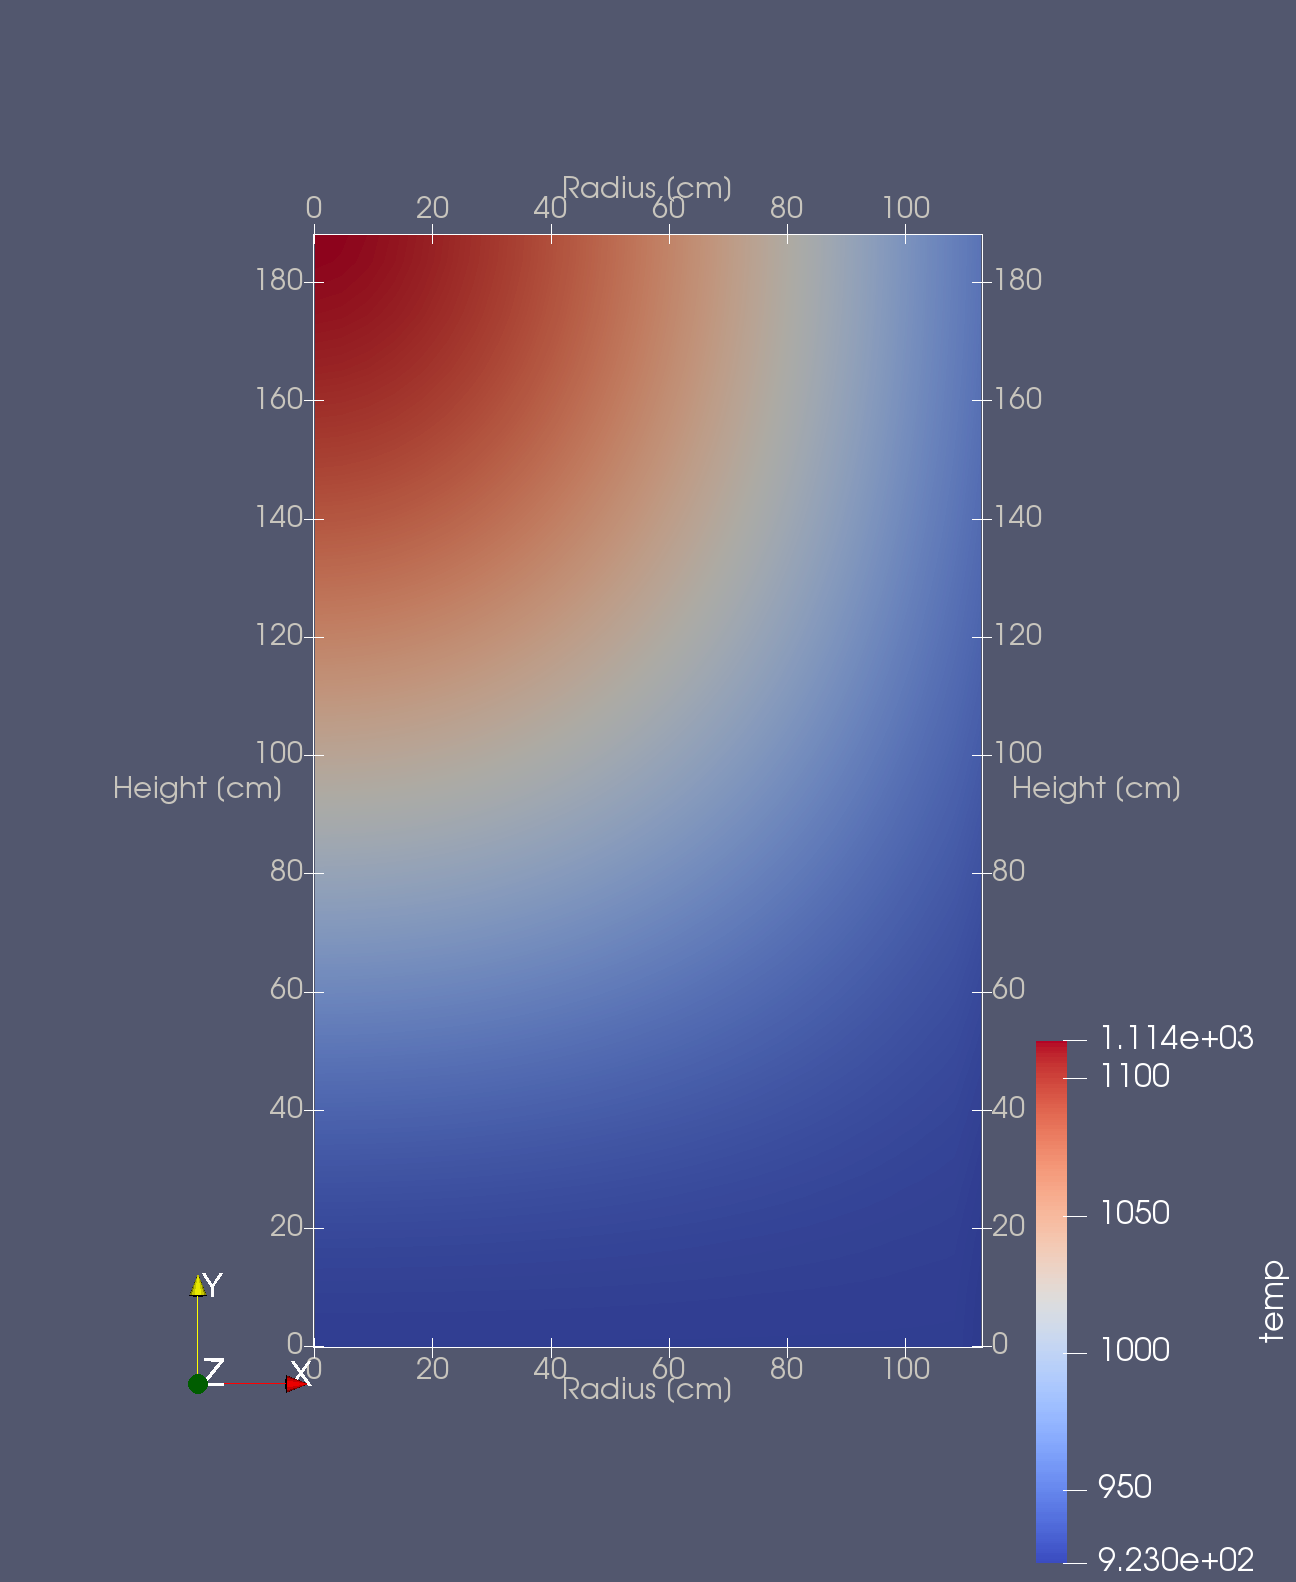
\includegraphics[width=.3\textwidth]{../paper/figures/eltemp}
				\end{subfigure}
				\begin{subfigure}
					\centering
					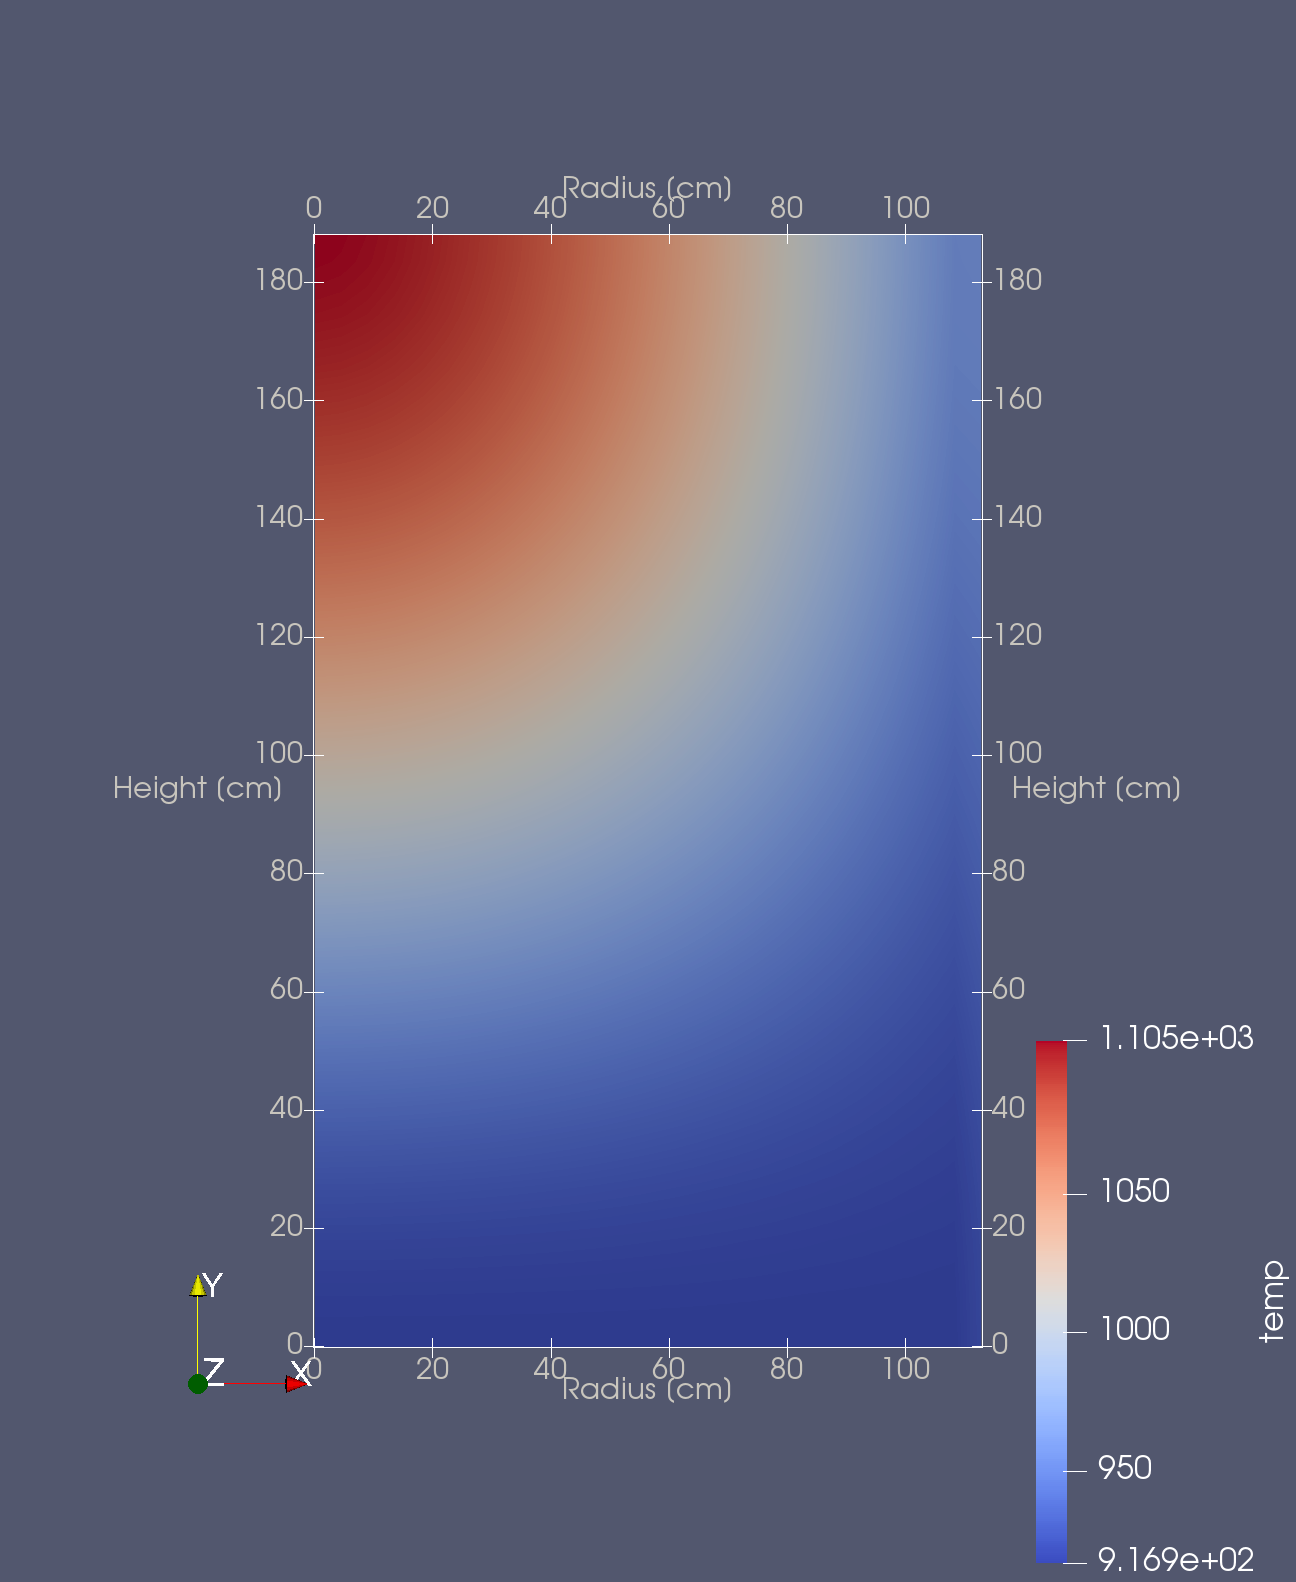
\includegraphics[width=.3\textwidth]{../paper/figures/eqtemp}
				\end{subfigure}\\
				\hspace*{\fill}
				(a) Start-up \hfill \hfill (b) Early-life \hfill \hfill
				(c) Equilibrium
				\hspace*{\fill}
				\caption{Temperature distribution in fuel salt region for
				start-up, early-life, and equilibrium fuel compositions.}
				\label{fig:temp}
			\end{figure}
		\end{columns}
\end{frame}

\begin{frame}
	\frametitle{Steady State}
		\begin{columns}
			\column[t]{5cm}
			\begin{table}[b]
				\small
				\centering
				\caption{Average fuel inlet temperature}
				\begin{tabular}{ll}
					\hline
					{Composition} & {Inlet temperature [K]}\\
					\hline
					Start-up & 964.85\\
					Early-life & 925.11\\
					Equilibrium & 916.85\\
					\hline
				\end{tabular}
				\label{table:inlet}
			\end{table}
			\column[t]{5cm}
			\begin{table}[b]
				\small
				\centering
				\caption{Average fuel outlet temperature}
				\begin{tabular}{ll}
					\hline
					{Composition} & {Outlet temperature [K]}\\
					\hline
					Start-up & 1067.40\\
					Early-life & 1025.39\\
					Equilibrium & 1016.67\\
					\hline
				\end{tabular}
				\label{table:outlet}
			\end{table}	
		\end{columns}
		
		\vspace{.3cm}
		\begin{itemize}
		\item Highest average inlet and outlet temperatures observed for the
		start-up composition, followed by early-life, and equilibrium
		compositions.
		\end{itemize}
\end{frame}

\begin{frame}
	\frametitle{Steady State}
		\textbf{\gls{DNP} Distribution}
		 \begin{figure}
		 	\centering
		 	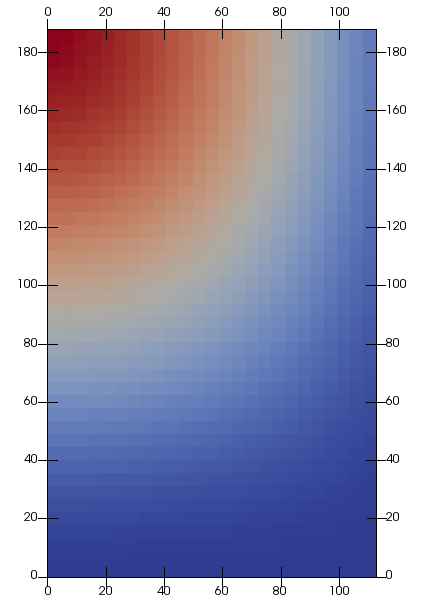
\includegraphics[width=.2\textwidth]{./images/pre1}
		 	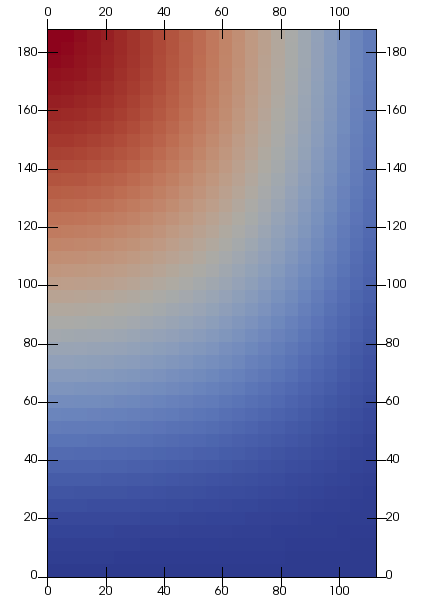
\includegraphics[width=.2\textwidth]{./images/pre2}
		 	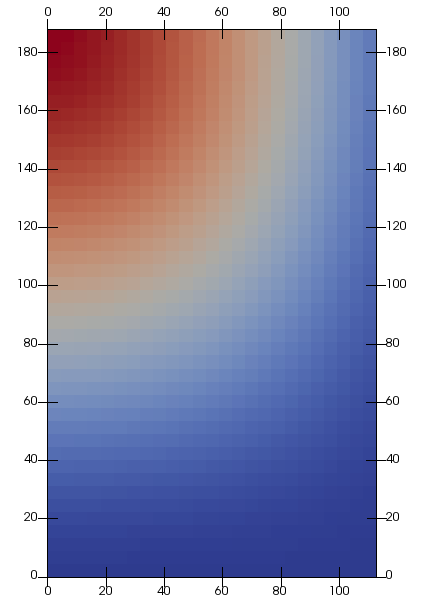
\includegraphics[width=.2\textwidth]{./images/pre3}
		 	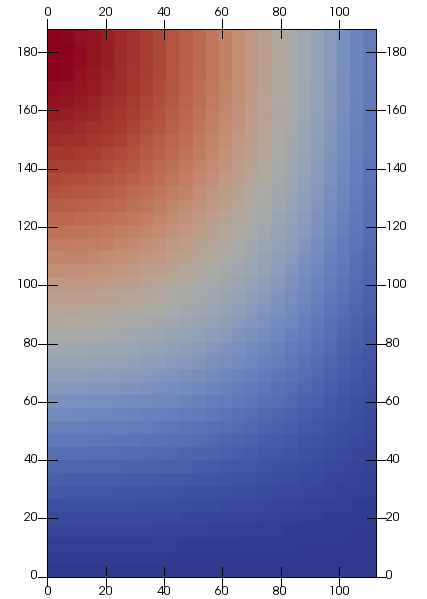
\includegraphics[width=.2\textwidth]{./images/pre4}\\
		 	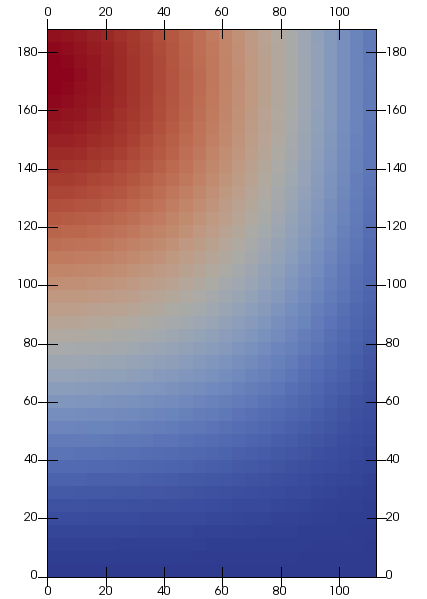
\includegraphics[width=.2\textwidth]{./images/pre5}
		 	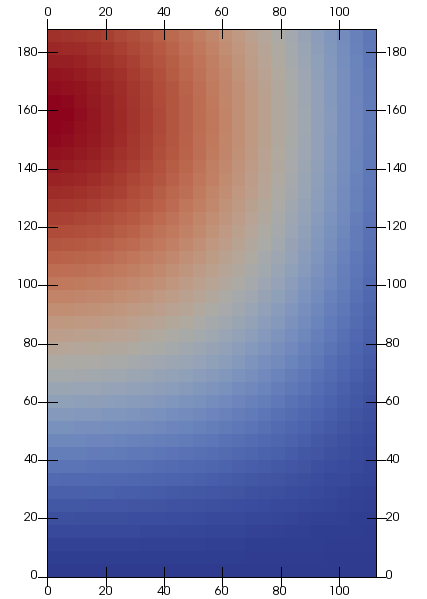
\includegraphics[width=.2\textwidth]{./images/pre6}
		 	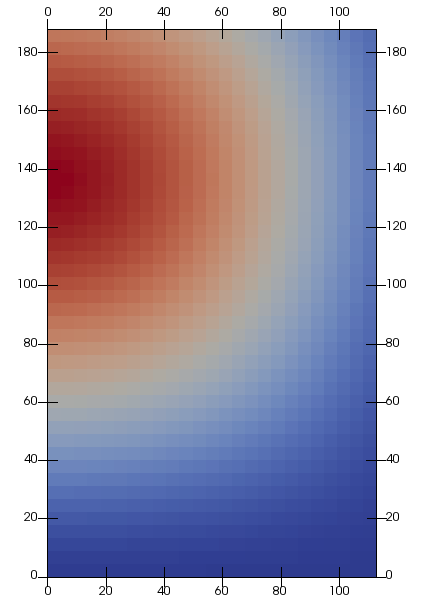
\includegraphics[width=.2\textwidth]{./images/pre7}
		 	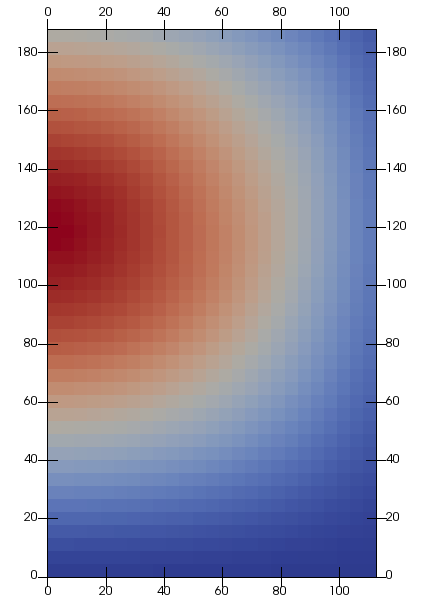
\includegraphics[width=.2\textwidth]{./images/pre8}
		 	\caption{\footnotesize \gls{DNP} distribution
		 	from group 1 to group 8 (left to right, top to bottom). $t_{1/2} =$
		 	55.60 s, 24.50 s, 16.30 s, 5.21 s, 2.37 s, 1.04 s, 0.42 s, and
		 	0.20 s.}
		 	\label{fig:dnp}
		 \end{figure}
\end{frame}
